% Created by tikzDevice version 0.12.6 on 2024-07-06 15:55:57
% !TEX encoding = UTF-8 Unicode
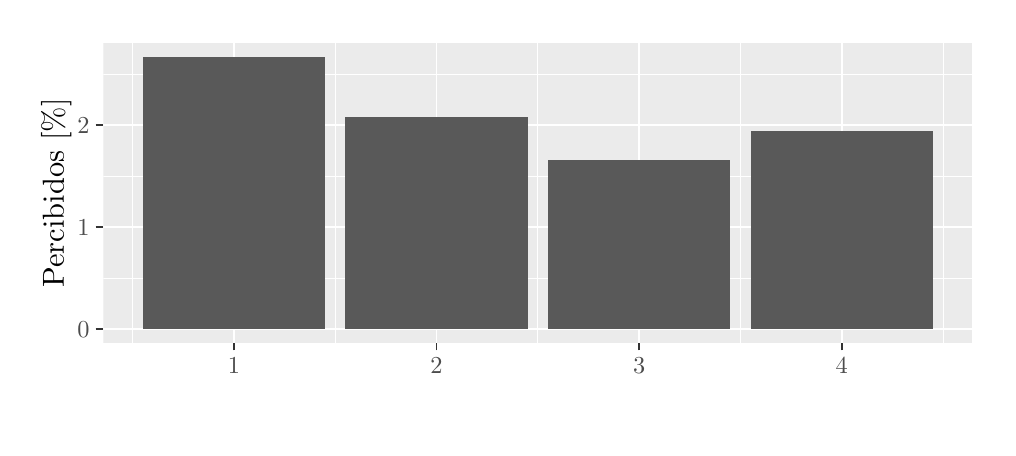
\begin{tikzpicture}[x=1pt,y=1pt]
\definecolor{fillColor}{RGB}{255,255,255}
\path[use as bounding box,fill=fillColor,fill opacity=0.00] (0,0) rectangle (346.90,144.54);
\begin{scope}
\path[clip] (  0.00,  0.00) rectangle (346.90,144.54);
\definecolor{drawColor}{RGB}{255,255,255}
\definecolor{fillColor}{RGB}{255,255,255}

\path[draw=drawColor,line width= 0.6pt,line join=round,line cap=round,fill=fillColor] (  0.00,  0.00) rectangle (346.90,144.54);
\end{scope}
\begin{scope}
\path[clip] ( 27.31, 30.69) rectangle (341.40,139.04);
\definecolor{fillColor}{gray}{0.92}

\path[fill=fillColor] ( 27.31, 30.69) rectangle (341.40,139.04);
\definecolor{drawColor}{RGB}{255,255,255}

\path[draw=drawColor,line width= 0.3pt,line join=round] ( 27.31, 54.04) --
	(341.40, 54.04);

\path[draw=drawColor,line width= 0.3pt,line join=round] ( 27.31, 90.91) --
	(341.40, 90.91);

\path[draw=drawColor,line width= 0.3pt,line join=round] ( 27.31,127.77) --
	(341.40,127.77);

\path[draw=drawColor,line width= 0.3pt,line join=round] ( 37.93, 30.69) --
	( 37.93,139.04);

\path[draw=drawColor,line width= 0.3pt,line join=round] (111.14, 30.69) --
	(111.14,139.04);

\path[draw=drawColor,line width= 0.3pt,line join=round] (184.35, 30.69) --
	(184.35,139.04);

\path[draw=drawColor,line width= 0.3pt,line join=round] (257.57, 30.69) --
	(257.57,139.04);

\path[draw=drawColor,line width= 0.3pt,line join=round] (330.78, 30.69) --
	(330.78,139.04);

\path[draw=drawColor,line width= 0.6pt,line join=round] ( 27.31, 35.61) --
	(341.40, 35.61);

\path[draw=drawColor,line width= 0.6pt,line join=round] ( 27.31, 72.47) --
	(341.40, 72.47);

\path[draw=drawColor,line width= 0.6pt,line join=round] ( 27.31,109.34) --
	(341.40,109.34);

\path[draw=drawColor,line width= 0.6pt,line join=round] ( 74.54, 30.69) --
	( 74.54,139.04);

\path[draw=drawColor,line width= 0.6pt,line join=round] (147.75, 30.69) --
	(147.75,139.04);

\path[draw=drawColor,line width= 0.6pt,line join=round] (220.96, 30.69) --
	(220.96,139.04);

\path[draw=drawColor,line width= 0.6pt,line join=round] (294.17, 30.69) --
	(294.17,139.04);
\definecolor{fillColor}{gray}{0.35}

\path[fill=fillColor] ( 41.59, 35.61) rectangle (107.48,134.11);

\path[fill=fillColor] (114.80, 35.61) rectangle (180.69,112.34);

\path[fill=fillColor] (188.02, 35.61) rectangle (253.91, 96.82);

\path[fill=fillColor] (261.23, 35.61) rectangle (327.12,107.18);
\end{scope}
\begin{scope}
\path[clip] (  0.00,  0.00) rectangle (346.90,144.54);
\definecolor{drawColor}{gray}{0.30}

\node[text=drawColor,anchor=base east,inner sep=0pt, outer sep=0pt, scale=  0.88] at ( 22.36, 32.58) {0};

\node[text=drawColor,anchor=base east,inner sep=0pt, outer sep=0pt, scale=  0.88] at ( 22.36, 69.44) {1};

\node[text=drawColor,anchor=base east,inner sep=0pt, outer sep=0pt, scale=  0.88] at ( 22.36,106.31) {2};
\end{scope}
\begin{scope}
\path[clip] (  0.00,  0.00) rectangle (346.90,144.54);
\definecolor{drawColor}{gray}{0.20}

\path[draw=drawColor,line width= 0.6pt,line join=round] ( 24.56, 35.61) --
	( 27.31, 35.61);

\path[draw=drawColor,line width= 0.6pt,line join=round] ( 24.56, 72.47) --
	( 27.31, 72.47);

\path[draw=drawColor,line width= 0.6pt,line join=round] ( 24.56,109.34) --
	( 27.31,109.34);
\end{scope}
\begin{scope}
\path[clip] (  0.00,  0.00) rectangle (346.90,144.54);
\definecolor{drawColor}{gray}{0.20}

\path[draw=drawColor,line width= 0.6pt,line join=round] ( 74.54, 27.94) --
	( 74.54, 30.69);

\path[draw=drawColor,line width= 0.6pt,line join=round] (147.75, 27.94) --
	(147.75, 30.69);

\path[draw=drawColor,line width= 0.6pt,line join=round] (220.96, 27.94) --
	(220.96, 30.69);

\path[draw=drawColor,line width= 0.6pt,line join=round] (294.17, 27.94) --
	(294.17, 30.69);
\end{scope}
\begin{scope}
\path[clip] (  0.00,  0.00) rectangle (346.90,144.54);
\definecolor{drawColor}{gray}{0.30}

\node[text=drawColor,anchor=base,inner sep=0pt, outer sep=0pt, scale=  0.88] at ( 74.54, 19.68) {1};

\node[text=drawColor,anchor=base,inner sep=0pt, outer sep=0pt, scale=  0.88] at (147.75, 19.68) {2};

\node[text=drawColor,anchor=base,inner sep=0pt, outer sep=0pt, scale=  0.88] at (220.96, 19.68) {3};

\node[text=drawColor,anchor=base,inner sep=0pt, outer sep=0pt, scale=  0.88] at (294.17, 19.68) {4};
\end{scope}
\begin{scope}
\path[clip] (  0.00,  0.00) rectangle (346.90,144.54);
\definecolor{drawColor}{RGB}{0,0,0}

\node[text=drawColor,rotate= 90.00,anchor=base,inner sep=0pt, outer sep=0pt, scale=  1.10] at ( 13.08, 84.86) {Percibidos [\%]};
\end{scope}
\end{tikzpicture}
